\chapter{Vulnerability overview}
Table \ref{tbl:vuln overview} depicts all vulnerabilities found during the penetration test. They are categorized by their risk and potential and are differentiated in the categories low, medium, high and critical. 

% Here describe what severities are and what do they mean in context of your report. It's better to keep the color code across all the report.

% Figure \ref{fig:vuln_overview} shows the overview of vulnerabilities grouped by target.

% \begin{figure}[h]
% \centering
% 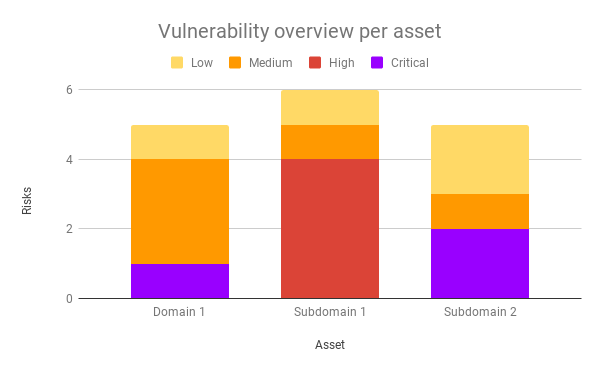
\includegraphics[width=\textwidth]{img/vuln_overview.png}
% \caption{Vulnerability overview}
% \label{fig:vuln_overview}
% \end{figure}

% \begin{table}[h]
% 	\begin{tabular}{| l | l | p{7cm} | l | l |}
% 		\hline 
% 		Risk & Asset & Vulnerability & Section & Page\\
% 		\hline 
% 		\cellcolor{codepurple}Critical & Domain 1 & Unauthenticated SQL Injection &  \ref{ss: issue-1} & \pageref{ss: issue-1} \\
% 		\hline 
% 		\cellcolor{red}High & Domain 1 & Stored XSS &  \ref{ss: issue-2}& \pageref{ss: issue-2}\\
% 		\hline 
% 		\cellcolor{orange}Medium & Subdomain 1 & Balance manipulation during order confirmation &  \ref{ss: issue-3} & \pageref{ss: issue-3} \\
% 		\hline 
% 		\cellcolor{yellow}Low & Subdomain 2 & Mail server misconfiguration & \ref{ss: issue-4} & \pageref{ss: issue-4} \\
% 		\hline
% 		\ldots & \ldots & \ldots & \ldots & \ldots \\
% 		\hline 
% 	\end{tabular}
% 	\caption{Vulnerability overview}
% 	\label{tbl:vuln overview}
% \end{table}
\begin{table}[h]
	\begin{tabular}{| l | l | p{8cm} | l | l |}
		\hline 
		Risk & Asset & Vulnerability & Section & Page\\
		\hline 
		\cellcolor{codepurple}Critical & SMB Server & Windows SMB Remote Code Execution &  \ref{ss: issue-1} & \pageref{ss: issue-1} \\
		\hline 
		\cellcolor{orange}Medium & 10.10.212.187:49663 & Sensitive Data Exposure &  \ref{ss: issue-2}& \pageref{ss: issue-2}\\
		\hline 
		\cellcolor{orange}Medium & SMB Share & Broken access control on SMB share &  \ref{ss: issue-3} & \pageref{ss: issue-3} \\
		\hline
		\cellcolor{orange}Medium & Host Device & Excessive Permissions &  \ref{ss: issue-3} & \pageref{ss: issue-3} \\
		\hline
		\cellcolor{yellow}Low & 10.10.212.187 & ASP.NET Version Disclosure & \ref{ss: issue-4} & \pageref{ss: issue-4} \\
		\hline
	\end{tabular}
	\caption{Vulnerability overview}
	\label{tbl:vuln overview}
\end{table}
The risk is calculated on the basis of 
\emph{\textbf{Common 
Vulnerability Scoring System}}(CVSS) Score
[\href{https://nvd.nist.gov/vuln-metrics/cvss#:~:text=The%20Common%20Vulnerability%20Scoring%20System,Base%2C%20Temporal%2C%20and%20Environmental.}{\textcolor{blue}{here}}].
It can be between 0 to
10, with 9-10 being the most severe and termed as critical.
These type of vulnerabilities along with
medium risk ones should be patched imeediately,
otherwise it could lead to huge loss in all sectors. For
example, these type of risks can lead to 
Personally Identifiable Information(PII), 
Sensitive Personally Identifiable Information(SPII) theft,
Denial of Service attacks, ransonware attacks etc. The 
company would have to incur high financial and trust loss
with these kind of attacks.
Next comes the
low risk ones, they doesn't affect the company in destructive way
but should be patched to avoid any issue in future.